\documentclass[12pt,a4paper,twoside,openright]{report}
	\usepackage[pdfborder={0 0 0}]{hyperref}    % turns references into hyperlinks
	\usepackage[margin=25mm]{geometry}  % adjusts page layout
	\usepackage{graphicx}  % allows inclusion of PDF, PNG and JPG images
	\usepackage{verbatim}
	\usepackage{docmute}   % only needed to allow inclusion of proposal.tex
	\usepackage{import} %import proposal from another folder
	\usepackage{pdfpages}
	\usepackage{listings}
	\usepackage{upquote}
	\usepackage{nameref}
	\usepackage{tikz}
	\usepackage{color}
	\usepackage[framemethod=tikz]{mdframed}
	\usepackage{courier}

	\definecolor{OliveGreen}{cmyk}{0.64,0,0.95,0.40}
	\definecolor{lightlightgray}{gray}{0.9}

	\usetikzlibrary{positioning}

	\lstset{
	language=[Objective]Caml,
	showstringspaces=false,
	breaklines=true,
	basicstyle=\normalsize\ttfamily,                 % Code font, Examples: \footnotesize, \ttfamily
	keywordstyle=\color{OliveGreen},        % Keywords font ('*' = uppercase)
	commentstyle=\color{gray},              % Comments font
	backgroundcolor=\color{lightlightgray}, % Choose background color
	}

	\surroundwithmdframed[
	hidealllines=true,
	backgroundcolor=lightlightgray,
	innerleftmargin=8pt,
	innertopmargin=0pt,
	innerbottommargin=0pt]{lstlisting}

	\raggedbottom                           % try to avoid widows and orphans
	\sloppy
	\clubpenalty1000%
	\widowpenalty1000%
	
	\renewcommand{\baselinestretch}{1.1}    % adjust line spacing to make
																					% more readable
	
	\begin{document}
	
	
	%%%%%%%%%%%%%%%%%%%%%%%%%%%%%%%%%%%%%%%%%%%%%%%%%%%%%%%%%%%%%%%%%%%%%%%%
	% Title
	
	
	\pagestyle{empty}
	
	\rightline{\LARGE \textbf{Charlie Crisp}}
	
	\vspace*{60mm}
	\begin{center}
	\Huge
	\textbf{Building a Blockchain Library for OCaml} \\[5mm]
	Computer Science Tripos -- Part II \\[5mm]
	Pembroke College \\[5mm]
	\today  % today's date
	\end{center}
	
	%%%%%%%%%%%%%%%%%%%%%%%%%%%%%%%%%%%%%%%%%%%%%%%%%%%%%%%%%%%%%%%%%%%%%%%%%%%%%%
	% Proforma, table of contents and list of figures
	
	\pagestyle{plain}
	
	\chapter*{Proforma}
	
	{\large
	\begin{tabular}{ll}
	Name:               & \bf Charlie Crisp                       \\
	College:            & \bf Pembroke College                     \\
	Project Title:      & \bf Building a Blockchain Library for OCaml \\
	Examination:        & \bf Computer Science Tripos -- Part II, July 2018  \\
	Word Count:         & \bf ????\footnotemark[1]\\
	Project Originator: & KC Sivaramakrishnan                    \\
	Supervisor:         & KC Sivaramakrishnan                    
	\end{tabular}
	}
	\stepcounter{footnote}
	
	
	\section*{Original Aims of the Project}
	
	To build a library in OCaml, which can be used as a building block for Blockchain applications. 
	The library should allow participating nodes to own a shared copy of a Blockchain data structure, agreed upon using consensus.
	Nodes should also be able to commit transactions to the blockchain, which should then be visible to other participating nodes. 
	
	
	\section*{Work Completed}
	
	All that has been completed appears in this dissertation.
	
	\section*{Special Difficulties}
	
	None
	 
	\newpage
	\section*{Declaration}
	
	I, Charlie Crisp of Pembroke College, being a candidate for Part II of the Computer
	Science Tripos, hereby declare that this dissertation and the work described in it are my own work,
	unaided except as may be specified below, and that the dissertation
	does not contain material that has already been used to any substantial
	extent for a comparable purpose.
	
	\bigskip
	\leftline{Signed}
	\bigskip
	\leftline{Date}
	
	\tableofcontents
	
	\listoffigures
	
	\newpage
	\section*{Acknowledgements}
	
	I would like to thank KC Sivaramakrishnan for being an extremely helpful supervisor throughout the duration of the dissertation, as well as over the past three years.\\
	I would also like to thank Anil Madhavapeddy for allowing me to use his laptop for the duration of the dissertation, and being a very supportive DoS.\\
	Finally I'd like to thank my friends and family for supporting me through my final year.
	
	%%%%%%%%%%%%%%%%%%%%%%%%%%%%%%%%%%%%%%%%%%%%%%%%%%%%%%%%%%%%%%%%%%%%%%%
	% now for the chapters
	
	\pagestyle{headings}
	
	\chapter{Introduction}
	Blockchain technology has existed for a long time, but the definition of 'blockchain' has changed drastically since its conception.
	Previously used just to describe a data structure, the term 'blockchain' is now widely used to also describe the accompanying consensus mechanisms.
	This is mainly due to the increasing popularity of cryptocurrencies such as Bitcoin \cite{Bitcoin} which use the 'Proof of Work' algorithm to solve the double spending problem \cite{}.
	However, whilst blockchain is undoubtedly the most important technology in the field of cryptocurrencies, where no single client can be trusted, it also has many uses outside this application.
	It can be used in other situations where clients can be trusted, for instance, a hospital maintaining medical records, or a bank wishing to record transactions from many of its own distributed clients.\\
	

	I have implemented a blockchain library in OCaml which allows the easy creation of blockchain applications.
	The blockchain is synchronised via a leader-based consensus mechanism with eventual consistency.
	Because the application is written in OCaml, it can be compiled to bytecode, unikernels or even javascript and is therefore suitable for a wide range of destination applications and devices.

	\section{The History of the Blockchain}
	The blockchain, in its simplest form, is a series of blocks of data, where each block contains the cryptographic hash of the previous block in the chain. 
	Figure \ref{fig:mainblockchain} is a graphical representation of a typical blockchain data structure.\\

	\begin{figure}
		\begin{center}
			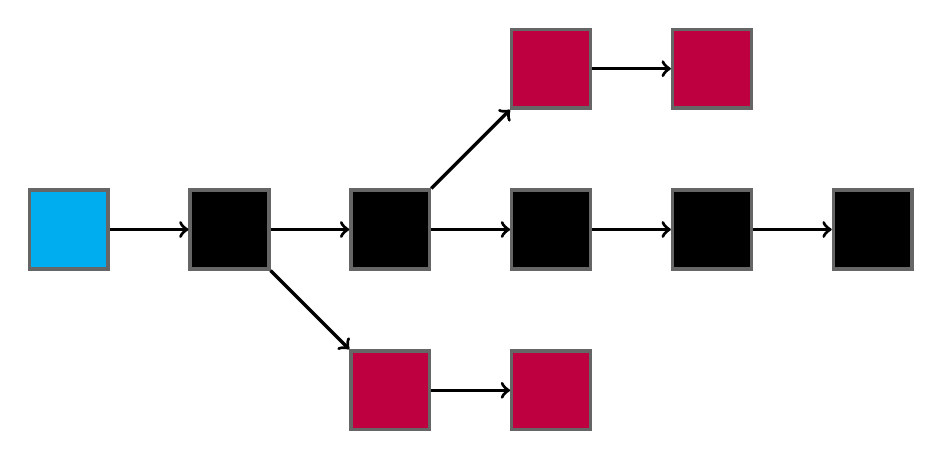
\begin{tikzpicture}[
				gennode/.style={rectangle, draw=black!60, fill=cyan!100, very thick, minimum size=10mm},
				mainnode/.style={rectangle, draw=black!60, fill=black!100, very thick, minimum size=10mm},
				subnode/.style={rectangle, draw=black!60, fill=purple!100, very thick, minimum size=10mm},
			]
			\node[gennode] (genesisblock) {};
			\node[mainnode] (block1) [right=of genesisblock] {};
			\node[mainnode] (block2) [right=of block1] {};
			\node[mainnode] (block3) [right=of block2] {};
			\node[mainnode] (block4) [right=of block3] {};
			\node[mainnode] (block5) [right=of block4] {};
			\node[subnode] (sub1) [below=of block2] {};
			\node[subnode] (sub2) [below=of block3] {};
			\node[subnode] (sub3) [above=of block3] {};
			\node[subnode] (sub4) [above=of block4] {};
			\begin{scope}[very thick, -stealth]
			\draw[->] (genesisblock.east) -- (block1.west);
			\draw[->] (block1.east) -- (block2.west);
			\draw[->] (block2.east) -- (block3.west);
			\draw[->] (block3.east) -- (block4.west);
			\draw[->] (block4.east) -- (block5.west);
			\draw[->] (sub3.east) -- (sub4.west);
			\draw[->] (block1.south east) -- (sub1.north west);
			\draw[->] (sub1.east) -- (sub2.west);
			\draw[->] (block2.north east) -- (sub3.south west); 
			\end{scope}
			\end{tikzpicture}
			\end{center}
		\caption{A typical blockchain structure}
		\label{fig:mainblockchain}
	\end{figure}
	The blockchain, as a cryptographically secure chain of blocks, was first conceptualised by Stuart Haber and W. Scott Stornetta in 1990 \cite{HaberStornetta}.
	However, until the creation of Git \cite{Git} in 2005, the blockchain was still a relatively niche concept.
	The invention of Bitcoin in 2008 is seen by many as the most pivotal moment in the history of blockchain technologies.
	Bitcoin uses the Proof of Work consensus algorithm to create a decentralised, trust-less, peer to peer network which is used to make transactions between virtual wallets.

	\section{Blockchain Today}
	At the time of writing, cryptocurrencies are generating both a huge amount of excitement and cynicism in popular media. 
	Cryptocurrencies aside from Bitcoin are paving the way to smarter uses of the blockchain.
	For example, Ethereum \cite{Ethereum} introduces the concept of Smart Contracts which allow the execution of code on the blockchain.\\
	
	Whilst it is possible to think of applications for blockchain technology in almost every sector, the development of applications outside the scope of crytocurrencies has been limited. 
	If one considers the example of OCaml, there are currently no libraries which allow a user to easily get started with building blockchain applications. \\

	\section{Work Completed}
	I have created a library which allows developers to create blockchain applications with the ease of importing a library.
	The project was designed to exist outside the realm of cryptocurrencies and therefore assumes that all participating nodes are trustworthy.
	Consensus is achieved by using a simple leader-based model where the leader node will periodically pull updates from all participating nodes and merge them into a central blockchain.
	This can then be viewed by all participating nodes, with the guarantee of eventual consistency.
	Setting up a network is as easy as specifying the location of the leader on all the participating nodes, and specifying the location of all participating nodes on the leader.\\
	
	I have evaluated the project by... FILL IN EVALUATION DETAILS

	\chapter{Preparation}
	Before starting work on the codebase for the project, I completed a lot of preparation in order to aid the development process later on.
	I spent some time learning to use OCaml and all of the different language features it provides.
	This was important because it allowed me to write idiomatic code which was not only powerful, but also easy to use by other developers.
	I also spent some time investigating a few key libraries, such as Irmin and Lwt.
	Understanding these libraries, the data structures they provide, and the technologies they present, allowed me to focus on the technological challenges in the project and not waste time reinventing the wheel. 
	Setting up a good development environment allowed me to run automated builds and, therefore, catch any errors in the code early.
	Lastly, I spent some time developing a requirements analysis for the final product. 
	This analysis helped drive the design and development of the blockchain library whilst not restricting the work that I was able to complete.

	\section{Starting Point}
		The project built upon functionality provided by Irmin [1] which is a distributed database system.  Irmin is fast, durable and has the branching capabilities which are required to build a blockchain.
		The project also made use of Ezirmin \cite{Ezirmin} which provides a simplified API to Irmin.

	\section{Using OCaml}
		At the start of the project, I had never used OCaml for any project of significance. 
		Whilst the first year Foundations of Computer Science course had given me some background into functional programming, there were still many key OCaml features which I had to learn.
		In the first few weeks of my project, I spent time studying the book Real World OCaml \cite{RealWorldOCaml} which proved a great introduction to many of OCaml's features.  

		\subsection{Pattern Matching}
		OCaml provides a very powerful syntax for matching patterns which allow you to write functions like the following\ldots 
		\begin{lstlisting}
type card = Card of string * int
let pattern_matcher_1 input = match input with 
  | Card("spades", 1) -> Printf.printf "It's the ace of spades!"
  | _ -> Printf.printf "Unlucky"
  
let pattern_matcher_2 = function 
  | Card(class, 1) -> Printf.printf "It's the ace of %s! class"
  | _ -> Printf.printf "Unlucky"
		\end{lstlisting}
		In the first example above, we have a function that will print a special string if it is passed the Ace of Spades. 
		Here, the pattern matching checks the that the tuple associated with the data type contains the string \texttt{spades} and the number 1.
		The second example uses the anonymous \texttt{function} keyword and matches the first argument of the tuple to the variable \texttt{class}.
		\subsection{Optionals}
		A built in data type that allows us to use the power of OCaml's pattern matching, is the \texttt{option}. 
		By using the \texttt{Some(\ldots)} and \texttt{None} constructors, one can create something of the type \texttt{'a option}. 
		This is comparable to the \texttt{null} type in languages such as Java, however as it is part of the type system, it forces the programmer to handle any cases where \texttt{null} could be returned.

		\subsection{Error Handling}
		OCaml provides multiple different ways of dealing with errors and exceptions. 
		A simple way of signifying an error in your return type, is to return an \texttt{option} which will be \texttt{None} if there is an error. 
		Whilst this can be inflexible for larger solutions, it also provides a quick and simple way of signifying that something has gone wrong.\\

		Another way of dealing with options in return types is to use the \texttt{bind} function:
		\begin{lstlisting}
val bind: 'a option -> ('a -> 'b option) -> 'b option = <fun>
		\end{lstlisting} 
		As the above type signature demonstrates, \texttt{bind} will take an \texttt{option} and apply a function to its contents if it exists, or return \texttt{None} otherwise.\\
		
		OCaml provides a built in type \texttt{Result.t} which is effectively an extention of optional return types, where the programmer is able to define arbitrary data to accompany the error type. The following code demonstrates a successful return type of \texttt{int} (with an unspecified \texttt{Error} type), and a \texttt{string} error type (with an unspecified \texttt{Ok} type).
		\begin{lstlisting}
# Ok 3;;
- : ('a, int) result = Ok 3
# Error "Something went wrong";;
- : (string, 'a) result = Error "Something went wrong";;
		\end{lstlisting} 

		\subsection{Polymorphic Variants}
		OCaml allows the programmer to define variant types such as the \texttt{Card} type that was defined earlier. This makes it very easy to make use of pattern matching with custom defined types.\\
		
		OCaml also introduces the notion of polymorphic variants which are more flexible and do not require an explicit type declaration.
		\begin{lstlisting}
# let card = `Card ("spades", 1);;
- : val card : [> `Card of string * int ] = `Card ("spades", 1)
		\end{lstlisting}
		Here, we have used a backtick to define a polymorphic type, and OCaml has automatically inferred a type. 
		The $>$ symbol acts as a lower limit on the tags that the variant \texttt{card} can take, i.e. it can have the tag \texttt{Card} or indeed other unspecified tags.
		When dealing with variant types as parameters, we may see the $<$ symbol in the type signature to denote that the parameter can only belong to given set of tags. The absence of both of these symbols indicates that a variant has exactly the given type signature. 

		\subsection{Modules and Functors}
		Modules provide a good way of grouping together related code in OCaml.
		They can be thought of as similar to traditional namespaces, although there a few key differences.
		OCaml also lets you define module type signatures which modules have to conform to.
		\begin{lstlisting}
module type Math = sig
  type t
  val add: t -> t -> t
  val subtract: t -> t -> t
end

module IntegerMath : Math with type t = int = struct 
  type t = int
  let add int1 int2 = int1 + int2
  let subtract int1 int2 = int1 - int2
end
		\end{lstlisting}
		The above code is a simple example where we have defined a module signature \texttt{Math} for adding and subtracting a custom type.
		The module \texttt{IntegerMath} is a module which adheres to this signature. 
		The slightly odd looking \texttt{with type t = int} serves the purpose of letting the compiler know that the type t is externally visible.
		Whilst in this example, we have used the trivial example of integer maths, it is easy to imagine this extending to, for example, matrices or sets where these functions are not built in.\\

		Modules are really useful for allowing the effective division of code into isolated units, however they are slightly inflexible. 
		Maybe we want to extract lower level details of the code in a module?
		In this case, we would have to create a whole new module for each possible implementation of this abstraction.
		An example of this could be a database that could use an in-memory or on-disc format for storing data.
		Functors allow us to create modules from other modules.
		\begin{lstlisting}
module Log(AO : Irmin.AO_MAKER)(V: Tc.S0) = struct
  ...
end
		\end{lstlisting}
		The above code is an example from the Ezirmin codebase (which we shall see later) where we define a functor which takes the module AO which is used for creating append only stores, and the module V which defines a data type.
		The result of this is a functor which can be used to create a Log module with either an in-memory or on-disc backend.
		\subsection{Development Environment}
		When developing a large scale system with OCaml, there are a couple of build systems available to use. 
		'jbuilder' \cite{jbuilder} is one of these systems which is becoming increasingly popular and is used daily by hundreds of developers.
		jbuilder allows the developer to specify arbitrary directory structures containing executables, libraries and more.
		I set up my project to build a blockchain library which included the interface for running both a Leader and Participant node. 
		I also defined two executables for running both the Leader and Participants in an example case. 
		I also used GNU Make \cite{GNUMake} to invoke jbuilder which allowed me to easily build and run any executables from the root of the directory.\\
		
		In order to ensure that the project would always build, I set up a continuous integration workflow using Travis-CI. 
		This was particularly useful as it ensured that whenever I pushed any updates to my GitHub repository, Travis would attempt to build the system and would notify me whenever there were any errors during the build.

	\section{Existing Libraries}
		This project is built on top of Irmin and Ezirmin.
		Irmin is a library that allow the creation of different types of data store, such as Read-Only, Append-Only and Read-Write.
		Ezirmin provides a simplified API for interacting with Irmin as well as providing the implementation of a mergeable log.
		Both Irmin and Ezirmin allow the use of different backends including an in-memory, and on-disc format. 
		The on-disc format uses the git protocol to store data, although an in depth exploration of this is left to the \nameref{Implementation} section.
		During the preparation stage of project, I spend some time familiarising myself with the API and codebases of these projects. 
		Being able to create dummy applications, and get a deeper understanding of the lower-level code was extremely useful later on when I encountered a few bugs which I had to work around.\\

		Another library which I spent some time familiarising myself with was Lwt \cite{Lwt}. 
		Lwt provides a way of interacting with threads in OCaml, although in Lwt they are known as 'Promises'.
		\begin{lstlisting}
val Lwt.return : 'a -> 'a Lwt.t 
val Lwt_main.run : 'a Lwt.t -> 'a
val Lwt.bind : 'a Lwt.t -> ('a -> 'b Lwt.t) -> 'b Lwt.t
		\end{lstlisting}
		The above code shows the basic functions for creating, running and combining threads.
		The above type \texttt{'a Lwt.t} refers to a thread which will eventually terminate with a value of type 'a, and follows the well established Monad design pattern.
		To elaborate on what these functions do, if we wish to obtain a thread which has already terminated with a value of type 'a, we can pass this value to \texttt{Lwt.return}, and it will happily oblige. If we wish to run a thread to completion and eventually return its value, then we can use \texttt{Lwt\_main.run}. Finally, if we wish to chain together two threads, we can use use \texttt{Lwt.bind} (or the infix notation \texttt{>>=}) to pass the result of the first thread onto a function which will return a second thread.

	\section{Requirements Analysis} \label{Requirements Analysis}
	During the preparation stage of my project, I spent some time analysing the requirements that would be suitable for my projects. This proved a good way of guiding the progress of the project and making sure that I solved all the problems that I set out to. Here, I will set out the criteria that I decided upon before starting development on the project.
	\subsection{Data Structure}
	A key component of this project was to build a blockchain data structure that would allow transactions to be added to a ledger. 
	From a participating node, it should be possible to add a transaction, of a given type, between two identities. 
	It should also be possible to view an ordered list of all transactions which currently exist in the blockchain.
	\begin{minipage}{\linewidth}
	\begin{lstlisting}
module type I_LogStringCoder = sig
  type t
  val encode_string: t -> string
  val decode_string: string -> t option
end

module type I_Config = sig
  type t
  module LogCoder: I_LogStringCoder with type t = t

  val validator: (t list -> t -> bool) option
end

module type I_Blockchain = sig
  type t

  val add_transaction_to_blockchain: t -> [> `Error | `Ok] Lwt.t
  val get_all_transactions: unit -> [> `Error | `Ok of t list] Lwt.t
  val get_transactions: int -> [> `Error | `Ok of t list] Lwt.t
end

module Make(Config: I_Config): I_Blockchain with type t = Config.t = struct 
  ...
end
	\end{lstlisting}
	\end{minipage}\\
	\\
	The above code is the technical specification that I used to define my project, and the functions complete the following operations:
	\begin{itemize}
		\item \texttt{I\_LogStringCoder} is a module that allows the user to specify arbitrary types to be stored on the blockchain, so long as they can be encoded to (and decoded from) a string.
		\item \texttt{I\_Config} contains information which is required to run the Blockchain.
			In particular, should the \texttt{validator} option contain the value \texttt{Some(f)}, then \texttt{f} will be a function that accepts a history of committed transactions, and validates whether a further transaction is valid. 
		\item \texttt{Make} is a functor which accepts a configuration module and will return a Blockchain module.
		\item \texttt{add\_transaction\_to\_blockchain} adds a user defined type to the blockchain and then return a polymorphic variant type containing information about whether the operation was successful. 
			This will return an error in the case that the transaction is not validated.
	\end{itemize} 

	\subsection{Consensus}
	Building consensus into the blockchain module was a key part of the project. 
	The actual design and development of the consensus algorithm was completed throughout the duration of the project and involved a lot of research into other consensus mechanisms.
	However, during the requirements analysis phase of the project I set out some goals for the final implementation.
	These goals were laid out in order to help drive the design and development of the consensus mechanism. 
	I decided on the following requirements:
	\begin{itemize}
		\item The consensus mechanism must guarantee eventual consistency. Strict consistency, although beneficial in some scenarios, is not required as it could add large overhead costs and is not necessary for all applications of the blockchain.
		\item The consensus mechanism must be scalable. Within the scope of this project, it should be possible for the blockchain to be shared by 4 or more nodes in a network. This should not hinder the performance of the system, and it should still be able to handle multiple successful transactions per second.
	\end{itemize}

	\chapter{Implementation} \label{Implementation}
	\section{The Blockchain Data Structure}
	Irmin is a library for OCaml providing data store functionality with a Git backend. 
	I used Irmin to build the blockchain data structure, however, this first required some analysis of the data models that Irmin exposes.
	I also did some research on Git to validate that it fulfilled the necessary criteria to be used as a blockchain.
	\subsection{Git as a blockchain}
		Git provides a data structure which can be interacted with via a command line API. However, it is not trivial why these data structure is classed as a blockchain. \\
		\\
		In order to convince oneself of this, it is worth considering what features are required for a data structure to be considered a blockchain. 
		Whilst there is no universally agreed definition of a blockchain, it is commonly accepted that it will exhibit the following features:
		\begin{enumerate}
			\item Data is stored in 'blocks'.
			\item Blocks are ordered.
			\item Each block contains a link to its parent block.
		\end{enumerate}
		Now we can consider the promises that Git makes and ensure that the above conditions are satisfied.
		\begin{enumerate}
			\item Git stores data as sequences of 'commits' which can be thought of as blocks.
			\item Git history is stored as a tree structure with arbitrary branching. This imposes an order on commits or blocks.
			\item Each Git commit contains the hash of the previous or parent commit.
		\end{enumerate}
		It is clear to see that Git has all the necessary properties to be used as a blockchain data structure.
	\subsection{Irmin}
		The next question that I needed to answer, was how it was best to interact with an underlying Git protocol, using OCaml. Irmin is a library for OCaml which provides Git-like, distributed, branchable storage \cite{Irmin}.\\
		\\
		Irmin uses a Git backend to store objects which immediately makes it suitable for use as a blockchain. However, it is also possible to consider Irmin's data store at a higher level. \\
		\\
		Irmin provides access to a Block Store and a Tag Store as shown in figure \ref{fig:IrminBlockStore}.
		\begin{figure}
			\begin{center}
			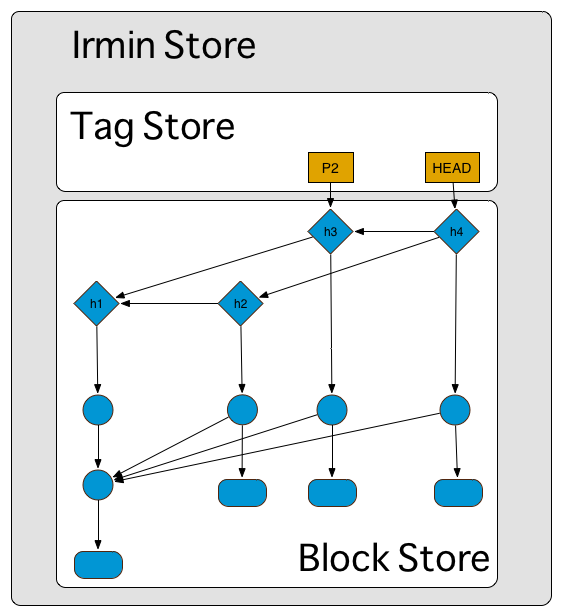
\includegraphics[width=8cm]{figs/irmin-stores.png}
			\caption{An Irmin Store composed of a mutable Tag Store and an immutable Block Store}
			\label{fig:IrminBlockStore}
			\end{center}
		\end{figure}
		The block store is an append-only store of immutable key-value pairs. Mutability comes from the tag store, which provides a way of mapping global branch names to blocks. Both of these stores combine to form an Irmin store with  promises which are beneficial for concurrency. For example, if a tag is not mutated, then you can be sure that the no change in the block store will be visible.\\
		\\
		Irmin Stores can be though of in terms of the following API, expressed in OCaml code. Here, we expose types for keys which address values, and tags which point to keys. The read and update functions allow us to interact with the block store. \\
		\begin{lstlisting}
  type t
  type tag
  type key 
  type value

  val read: t -> ?branch:tag -> key -> value option
  val update: t -> ?branch:tag -> key -> value -> unit
			
		\end{lstlisting}
		Amongst other different interfaces, Irmin provides a built in API for interacting with an append-only store. This key functionality of this module is expressed in the following code, where \texttt{mem} checks for the presence of a key, \texttt{find} reads values, and \texttt{add} writes to the store.

		\begin{lstlisting}
  val mem: t -> key -> bool Lwt.t
  val find: t -> key -> value option Lwt.t
  val add: t -> value -> key Lwt.t
		\end{lstlisting}
	\subsection{Ezirmin}
	Ezirmin is a library that provides a simplified interface to the Irmin library. It is designed to provide a interface to Irmin without functors, but with some useful defaults. Importantly, it has a built in log data structure which uses Irmin's append-only store, saved on disk in the git format.\\
	\begin{lstlisting}
module type FS_Log = sig
  type elt 
  type cursor 
  val append : ?message:string -> branch -> path:string list -> elt -> unit Lwt.t
  val get_cursor : branch -> path:string list -> cursor option Lwt.t
  val read : cursor -> num_items:int -> (elt list * cursor option) Lwt.t
  val read_all : branch -> path:string list -> elt list Lwt.t
  ...
end
	\end{lstlisting}
	The above code gives some of the interface for an Ezirmin log which uses a file system backend.
	The log allows for items to be appended to and read from a log.
	In particular, the function \texttt{read} will read from the position of a cursor into the log, and will return a new cursor for the next unread log item, alongside the result.
	This interface therefore provides all the functionality required to build a blockchain.
	
	\section{Consensus Algorithms}
	Building consensus was by far the most important part of work completed for this project. 
	In order to guide the design of the consensus mechanism, I completed an extensive amount of research on existing algorithms
	This section will briefly summarise this research and my conclusions about their suitability for the project. 
	The resulting design for consensus is a leader based approach, where participant nodes can commit transactions to a mempool.
	This mempool is then polled for updates by the leader, and these updates are then validated and committed to the main blockchain.
	This blockchain can be read by all participants, and provides a definitive source of ordered, committed transactions.

		\subsection{Building Consensus}
			\subsubsection*{Proof of Work}
			%TODO: Use a diagram,
			Proof of Work (PoW) is a deceptively simple consensus mechanism, used by most cryptocurrencies to avoid the double spending problem.
			Transactions are contained within blocks which can be broadcast out to the network of participating nodes. 
			Whenever a block is received by a participating node, the node checks that the block contains a proof of computational work done. 
			This proof usually takes the form of a random sequence of data (this is known as a nonce) appended to the end of the block, causing the block's hash to be prefixed with a set number of 0s.
			This acts as a proof of computational work, because the data appended to the end of a block can only be found by a brute force method called mining, but can also be verified easily by simply computing the block's hash.\\
			
			Why is this useful? 
			Well, this allows us to make guarantees on the validity of the blockchain based on the simple assumption that more that 50\% of the workforce is genuine.
			If we assume that the longest chain of blocks is the correct one, then in order to create a sequence of biased transactions, we would have to create a chain longer than the correct one. 
			This would require an equal number of 'Proof of Work's, which, due to the random nature of block mining, would require more than 50\% of the workforce.
			Whilst it may be possible to maintain an equally sized chain with less that 50\% of the workforce for a short period of time, the chances of this decrease rapidly as time passes.
			All in all this means that the longer a block has been in the chain, the more likely it is that the block is valid.\\

			Whilst this forms a very effective mechanism for achieving consensus, there are also some considerable downsides to using a PoW approach to consensus. 
			Firstly, there is a huge amount of computational work wasted in the process of mining. 
			The effect of this is energy consumption \cite{BitcoinEnergy} and wastage to a level which can cause serious environmental harm.
			PoW also does not generalise well outside of the scope of cryptocurrencies.
			It assumes no trust in any participants which may not be a suitable model for an application. 
			Additionally, it also assumes that miners can be rewarded, usually with cryptocurrency, but this incentive is ad hoc and may not exist in other applications.
			
			\subsubsection*{Mempools}
			Mempools are an important part of the design of Bitcoin, and whilst they are not inherently linked to the Proof of Work consensus algorithm, they are worth investigating. 
			When a Bitcoin transaction is made, it is first written into what is known as a Mempool. 
			This transaction can then be seen by participating miners, who can then choose to put this in the next block that they mine. 
			This is significant, as it provides a 'waiting room' for any transactions that have not yet been validated.  

			\subsubsection*{Proof of Stake}
			The Proof of Stake (PoS) algorithm is used by some cryptocurrencies and works by randomly allowing participants to create (or 'forge') a single block.
			However, the probability that a participant is chosen to 'forge' a block, is weighted by its stake, such that participants with higher stakes in the blockchain are more likely to be chosen to forge a block.\\

			So, why is PoS desirable? 
			By far the most convincing reason for using PoS over PoW, is that there is no need to waste lots of energy in the process of mining. 
			This hugely reduces the environmental impacts of scaling a PoS network.
			Using PoS also allows trust to be distributed according to an arbitrary heuristic which can be desirable property in some applications.\\

			One of the flaws of PoS is that it does not have such a strong deterrent against attacks.
			With PoW, attacks require huge amounts of computational power and it is likely that to create an attack, you would have to spend more on hardware than you would gain. 
			PoS doesn't have this same built in mechanism, and so there have been many suggested schemes for increasing the safety of PoS networks.
			For example, it is possible that participants should need to pay some form of deposit before forging blocks, which can be slashed if they break any rules. 
			PoS also suffers from the same problem as PoW in that it does not generalise well. 
			It is another example of a consensus mechanism designed for networks with a strong notion of Stake and with minimal trust in any individual participant.

			\subsubsection*{Paxos}
			Paxos is a family of consensus protocols which can be used to guarantee consistency in distributed systems. 
			It was first proposed in a paper by Leslie Lamport in 1998 \cite{Paxos}, although the paper was first submitted in 1990.
			Named after a fictitious civilisation living on the island of Paxos, the algorithm puts forward a way for any number of nodes to propose and agree on a value.
			Participating nodes belong to various roles, one of which is known as a 'Proposer' or Leader.\\

			The main part of the algorithm is split into two sections, propose and accept.
			In the first stage, a Proposer decides that it wants to propose a value and then broadcasts out a 'Prepare' message to a quorum of 'Acceptors'.
			Acceptors will then decide if they want to make a 'Promise' which is a commitment to accepting that proposal in the future. 
			If a quorum of promises is received by the Proposer, then it will assign a value to its proposal and will again send an 'Accept Request' out to a quorum of Acceptors.
			Finally, if enough 'Accept' messages are received then the Proposer can be certain that the value has been agreed upon by consensus.\\

			This algorithm has been proved to be consistent but it also has a lot of complexity and a lot of different variants. 
			The combination of different roles and states makes it easy to implement incorrectly.
			It is also important to consider that Paxos describes a 'family' of algorithms, with some parts left deliberately unspecified, and choosing how to implement these is not a trivial decision.
			The final issue with Paxos is that it cannot guarantee progress.
			Whilst it enforces conditions which make it unlikely that progress will not be made, it is still theoretically possible for the mechanism to stall indefinitely.

			\subsubsection*{Raft}
			%TODO: Finish description of Raft and it's concept of terms.
			Raft \cite{Raft} is an algorithm that was designed to be equivalent and as efficient as Paxos, however, it also places a much greater emphasis on comprehensibility.
			It uses the notion of a \textit{strong leader}, which is an elected server that has total control over which log entries are accepted.
			There are two other types of server, a \textit{follower} and a \textit{candidate}. 
			Followers are completely passive, and only respond to requests from leaders and candidates. 
			A candidate is a server that has put itself forward for election.\\

			So how does the algorithm operate? 
			Time in Raft is split into \textit{terms} which are labelled by a monotomically increasing integer. 
			Each term effectively signals a time period where a particular server is the leader. 
			A term starts with a leadership election when a follower transitions into the candidate state, increments its term number and requests votes from other servers. 
			It will wait for a majority of votes and then elect itself the leader, unless it times out or receives a message from another leader with a greater term number. 
			Typically, these leader election processes are triggered when a follower doesn't receive a heartbeat message from the leader for longer than a given time.
			In the pathological case, the vote can be split between leaders, triggering a new election which is also split and so on.
			However, Raft uses randomised election timeouts to avoid this problem.
			Additionally, Raft also prescribes some restrictions on the servers which can be elected leader so as to avoid newly elected leaders overwriting previously appended log items.\\
			
			Raft is an simple algorithm that is easy to understand, but it also guarantees the Log Matching Property that if two logs contain a log entry with the same index and term, then that entry, and all preceding entries will be identical.

		\subsection{A New Approach}
		I have build a consensus mechanism that uses a mempool and a simple leader based algorithm. 
		Because I have implemented a centralised algorithm, my specification has differed slightly from that presented in the \nameref{Requirements Analysis} to take into account differing functional requirements for a leader and for a participant.
		As I am assuming that all participating nodes can be trusted, it is possible to use a leader based approach without introducing security issues such as the ones tackled by the Proof of Work mechanism. 
		This approach also reduces the potential complexity of implementing completely decentralised consensus.
		My approach makes use of the mergeable log data structure provided by Ezirmin, and the synchronisation module that allows updates from a log to be pulled into another.
		Finally, I have introduced the notion of validation which allows both participants and leader nodes to accept or reject transactions depending on arbitrary conditions.
		
			\subsubsection*{Leaders}
			My consensus mechanism uses the notion of a \textit{strong leader} similar to that used by the Raft protocol. 
			The leader is chosen statically in order to reduce the complexity of implementation, and it also has a statically defined list of \texttt{remotes} which specifies the location of all participants.
			The leader is a node which will never actually request transactions to be added to the blockchain, its role is simply to periodically read requests from the mempools of participants, validate them, and then add them to the blockchain.
			This blockchain can be read by any participant, and is treated as the empirical source of which transactions have been committed and in which order. 
			That is, any two nodes that read a copy of the blockchain, will always agree on content and ordering of log items in the blockchain, up until the end of the shortest copy (or both copies).\\

			\begin{lstlisting}
module type I_LeaderConfig = sig
  type t
  module LogCoder: Participant.I_LogStringCoder with type t = t    
  val remotes: string list
  val validator: (t list -> t list -> t list) option
end
module type I_Leader = sig
  val init_leader: unit -> (unit -> unit Lwt.t) Lwt.t
end
module MakeLeader (Config: I_LeaderConfig) : I_Leader = struct
  ...
end
			\end{lstlisting}

			The above code is the specification of the leader module, which differs slightly from the centralised specification presented in the \nameref{Requirements Analysis}.
			In particular, the \texttt{init\_leader} function will perform an initialisation step, and then return a function which, when executed, will actually start the consensus process.

			\subsubsection*{Participants}
			Participants, in contrast to leaders, can request transactions to be added to the blockchain. 
			This is done by writing a transaction to a local mempool, which is then read by the leader.
			Validation can of this transaction can also happen at this stage, but as we'll see later, it cannot filter out all invalid transactions, and only exists to ease load on the leader.\\

			\begin{lstlisting}
module type I_LogStringCoder = sig
  type t
  val encode_string: t -> string
  val decode_string: string -> t option
end
module type I_ParticipantConfig = sig
  type t
  module LogCoder: I_LogStringCoder with type t = t
  val leader_uri: string option
  val validator: (t list -> t -> bool) option
end
module type I_Participant = sig
  type t
  val add_transaction_to_mempool: t -> [> `Could_Not_Pull_From_Remote | `Validation_Failure | `Ok] Lwt.t
  val get_transactions_from_blockchain: int -> [> `Error | `Ok of t list] Lwt.t
  val get_all_transactions_from_blockchain: unit -> [> `Error | `Ok of t list] Lwt.t
end
module Make(Config: I_ParticipantConfig): I_Participant with type t = Config.t = struct
  ...
end
			\end{lstlisting}

			The above specification shines a light on the role of participants and the functionality they provide.
			The module includes the ability to define custom data types that can be stored on the blockchain, to define how to validate transactions, to read from the blockchain, and to attempt to write to the blockchain by writing to a mempool.

			\subsubsection*{Retrieving local updates}
			The mechanism used by the leader to read mempool updates is different for the situations when the participant is on the same machine, and when it is on a remote machine. 
			Here, I will detail the process of reading updates from a participant on the same machine as the leader.\\

			\begin{figure}
				\begin{center}
					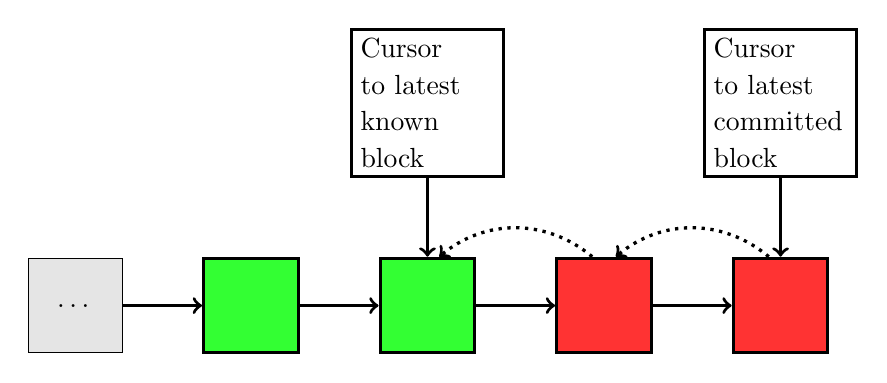
\begin{tikzpicture}[
						known/.style={rectangle, draw=black!100, fill=green!80, very thick, minimum size=12mm},
						mainnode/.style={rectangle, draw=black!100, fill=red!80, very thick, minimum size=12mm},
						label/.style={rectangle, draw=black!100, fill=black!0, very thick, minimum size=5mm, text width=1.7cm},
						invis/.style={rectangle, draw=black!100, fill=black!10, minimum size=12mm}
					]
					\node[invis] (invis) {\ldots};
					\node[known] (block1) [right=of invis] {};
					\node[known] (block2) [right=of block1] {};
					\node[label] (label1) [above=of block2] {Cursor to latest known block};
					\node[mainnode] (block3) [right=of block2] {};
					\node[mainnode] (block4) [right=of block3] {};
					\node[label] (label2) [above=of block4] {Cursor to latest committed block};
					\begin{scope}[very thick, -stealth]
					\draw[->] (invis.east) -- (block1.west);
					\draw[->] (label1.south) -- (block2.north);
					\draw[->] (block1.east) -- (block2.west);
					\draw[->] (block2.east) -- (block3.west);
					\draw[->] (block3.east) -- (block4.west);
					\draw[->] (label2.south) -- (block4.north);
					\path[dotted, ->] (block4.north)+(-1.5mm,0) edge  [bend right=40]  ([xshift=1.5mm]block3.north);
					\path[dotted, ->] (block3.north)+(-1.5mm,0) edge  [bend right=40]  ([xshift=1.5mm]block2.north);
					\end{scope}
					\end{tikzpicture}
					\end{center}
				\caption{A mempool on a local participant}
				\label{fig:readlocalpartudpates}
			\end{figure}

			The leader will always maintain a cursor to the latest entry it has read from the participant mempool.
			When it attempts to find new updates, it will get a new cursor to the latest element of the mempool.
			The leader can then compare these two cursors, and if the \textit{latest known} cursor points to an entry with an earlier timestamp than the \textit{latest} cursor, then it will add the \textit{latest} item to an accumulator, and then repeat the process with a cursor pointing to the parent of the \textit{latest} node. 
			Finally, when the cursors match, the items in the accumulator are returned as new updates which can be added to the leader mempool and the \textit{latest known} cursor is updated accordingly.
			It is important to note that no validation is performed at this stage as no item has been added to the blockchain yet.
			Figure \ref{fig:readlocalpartudpates} shows how unseen (red) blocks are read sequentially until the seen (green) blocks are reached.
	\chapter{Evaluation}
	
	\chapter{Conclusion}
	
	
	%%%%%%%%%%%%%%%%%%%%%%%%%%%%%%%%%%%%%%%%%%%%%%%%%%%%%%%%%%%%%%%%%%%%%
	% the bibliography
	\bibliographystyle{acm}
	\bibliography{refs}
	\addcontentsline{toc}{chapter}{Bibliography}
	
	%%%%%%%%%%%%%%%%%%%%%%%%%%%%%%%%%%%%%%%%%%%%%%%%%%%%%%%%%%%%%%%%%%%%%
	% the appendices
	\appendix

	\chapter{Project Proposal}
	
	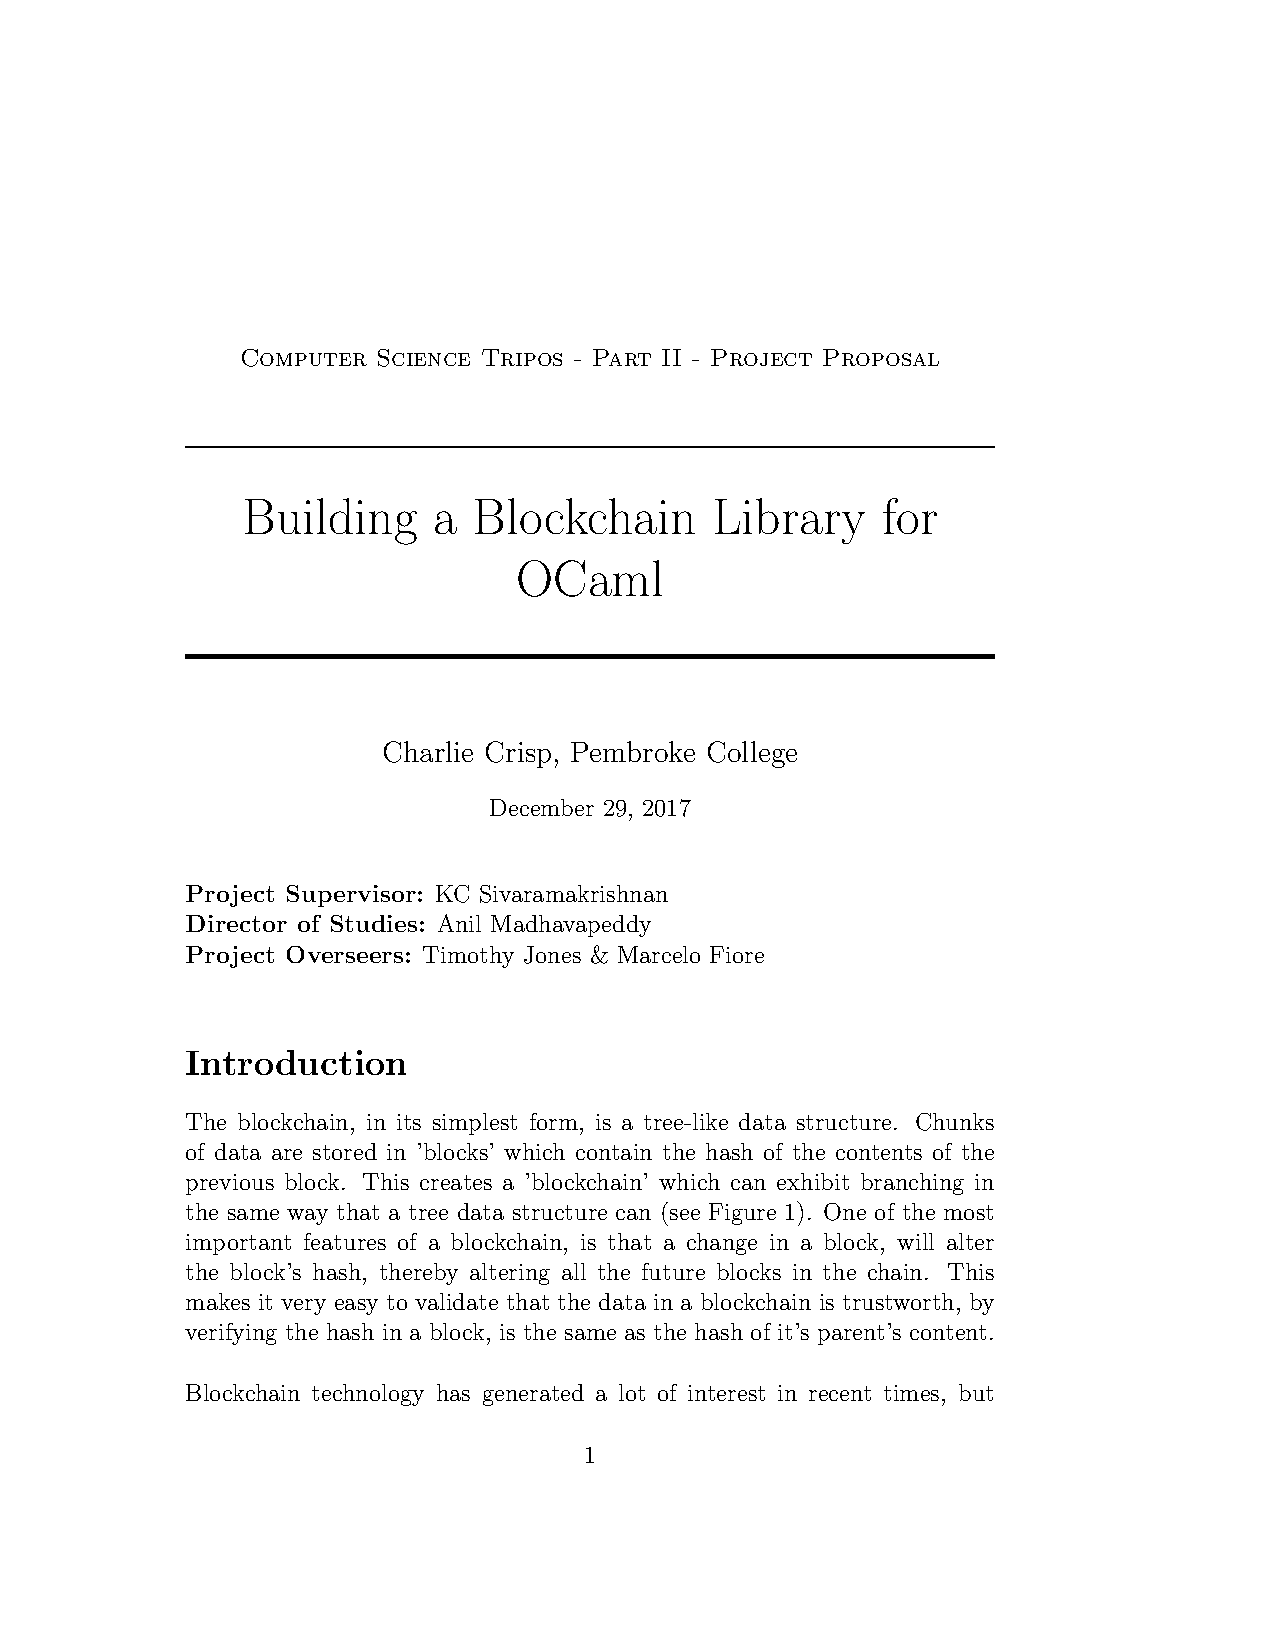
\includepdf[pages=-]{Part_II_Project_Proposal_Draft.pdf}
	
	\end{document}